
\documentclass[10pt]{exam}
\usepackage{graphicx}
\usepackage{listings}

\newcommand{\R}{\mathbb{R}}
\newcommand{\changes}[1]{{\color{red} #1}}
\usepackage{xcolor}
\usepackage[english]{babel}
\usepackage{amsmath,amssymb,amsthm,mathdots}
\usepackage{graphicx}
\usepackage[colorinlistoftodos]{todonotes}


\renewcommand{\thequestion}{\arabic{question} }
\renewcommand\questionlabel{\llap{\thequestion)}}


\usepackage{xcolor}
\definecolor{SolutionColor}{rgb}{0.1,0.3,1}

\unframedsolutions
\shadedsolutions
\definecolor{SolutionColor}{rgb}{0.9,0.9,1}
\renewcommand{\solutiontitle}{\textbf{Solution}$:\>$  }




%Mathcal and 
\newcommand{\mb}[1]{\mathbb{#1}}
\newcommand{\mc}[1]{\mathcal{#1}}

%Various possibilities for norms
\newcommand{\norm}[2]{\|#1\|_{#2}}
\newcommand{\normtwo}[1]{\|#1\|_{2}}
\newcommand{\normp}[1]{\|#1\|_{p}}

\newcommand{\rn}{\mathbb{R}^n}
\newcommand{\rnn}{\mathbb{R}^{n\times n}}
\newcommand{\rmn}{\mathbb{R}^{m\times n}}



%Boldface for vectors and tildes
\renewcommand{\vec}[1]{{#1}•}
\newcommand{\mat}[1]{{#1}•}

\newcommand{\vect}[1]{\widetilde{\boldsymbol{#1}}}
\newcommand{\matt}[1]{\widetilde{\boldsymbol{#1}}}

%Column and row equivalence
\newcommand{\roweq}{\stackrel{\text{row}}{\sim}}
\newcommand{\coleq}{\stackrel{\text{col}}{\sim}}

\newtheorem{definition}{Definition}
\newtheorem{example}{Example}
\newtheorem{fact}{Fact}
\newtheorem{remark}{Remark}


%Vector spaces
\newcommand{\rank}{\text{rank}\,}
\renewcommand{\dim}{\text{dim}\,}
\newcommand{\Span}[1]{\text{Span}\,\{#1\}}
\newcommand{\basis}[1]{\left\{ #1\right\}}


%Matrix environments
\newcommand{\bmat}[1]{\begin{bmatrix}#1\end{bmatrix}}
\newcommand{\pmat}[1]{\begin{pmatrix}#1\end{pmatrix}}
\newenvironment{amatrix}[1]{%
  \left(\begin{array}{@{}*{#1}{c}|c@{}}
}{%
  \end{array}\right)
}


%Trace and determinant
\newcommand{\diag}{\mathsf{diag}\,}
\newcommand{\range}{\mathsf{range}\,}
\newcommand{\trace}{\mathsf{trace}\,}


\usepackage{hyperref}
\title{MA 402: Project 5}
\date{}
\begin{document}
\maketitle
\textbf{Instructions}: 

\begin{itemize}
\item Detailed instructions regarding submission are available on the class website\footnote{\url{https://github.ncsu.edu/asaibab/ma402/blob/master/project.md}}.
\item The zip file should contain three files hw5.pdf, hw5.tex, classnotes.sty. 

\end{itemize}

\vspace{2mm}

\begin{questions}

\question [20] Consider the function \changes{$f(x) = x$} in the interval $[0,2\pi)$. 
\begin{parts}
\part Derive the Fourier coefficients $c_k$ for $k=0,\pm 1,\pm 2,\dots$.
\begin{align*}
    c_0 &= \frac{1}{2\pi}\int_0^{2\pi}x\ dx\\
        &= \frac{1}{2\pi}\left[\frac{x^2}{2}\right]\biggr\rvert_0^{2\pi}\\
        &= \frac{1}{2\pi}\frac{4\pi^2 - 0}{2}\\
        &= \pi\\
        \\
    c_k &= \frac{1}{2\pi}\int_0^{2\pi}xe^{-ikx}\ dx,\ k=\pm 1,\ \pm 2, ...\\
        &= \frac{1}{2\pi}\left[\frac{xe^{-ikx}}{(-ik)} - \frac{e^{-ikx}}{(-ik)^2}\right]\biggr\rvert_0^{2\pi}\\
        &= \frac{1}{2\pi}\left(\frac{2\pi}{-ik} + \frac{1}{k^2} - \frac{1}{k^2}\right)\\
        &= \frac{1}{-ik}\\
        &= \frac{i^4}{i^3k}\\
        &= \frac{i}{k}
\end{align*}

\part Derive the Fourier coefficients $a_0,a_k,b_k$ for $k=1,2,\dots,$.
\begin{align*}
    a_0 &= c_0\\
        &= \pi\\
        \\
    a_k &= c_k + c_{-k}\\
        &= \frac{i}{k} + \frac{i}{-k}\\
        &= 0\\
        \\
    b_k &= i(c_k - c_{-k})\\
        &= i\left(\frac{i}{k} - \frac{i}{-k}\right)\\
        &= i\frac{2i}{k}\\
        &= \frac{-2}{k}\\
\end{align*}

\part Plot the partial Fourier series, along with the function $f$, by retaining $n=1,10,50,100$ terms in the summation (use the second form involving cosines and sines).
\begin{lstlisting}[language = Python]
import numpy as np
import matplotlib.pyplot as plt

def problem1c(x, k):
  a0 = np.pi
  f = a0
  for i in range(1,k+1):
    bi = -2/i
    f += bi*np.sin(i*x)
  return f

resolution = 200
x = np.linspace(0,2*np.pi, resolution)

nrange = (1,10,50,100)

_, ((ax1,ax2),(ax3,ax4)) = plt.subplots(2,2,figsize=(10,10))
axes = (ax1,ax2,ax3,ax4)

for i in range(4):
  k = nrange[i]
  ax = axes[i]
  ax.plot(x,x,label='f(x)')
  ax.plot(x,problem1c(x,k),label='Fourier Approximation')
  ax.set_title('n = %d' % k)
  ax.legend()
  
ax1.set_ylabel('f(x)')
ax3.set_ylabel('f(x)')
ax3.set_xlabel('x')
ax4.set_xlabel('x')
plt.show()
\end{lstlisting}

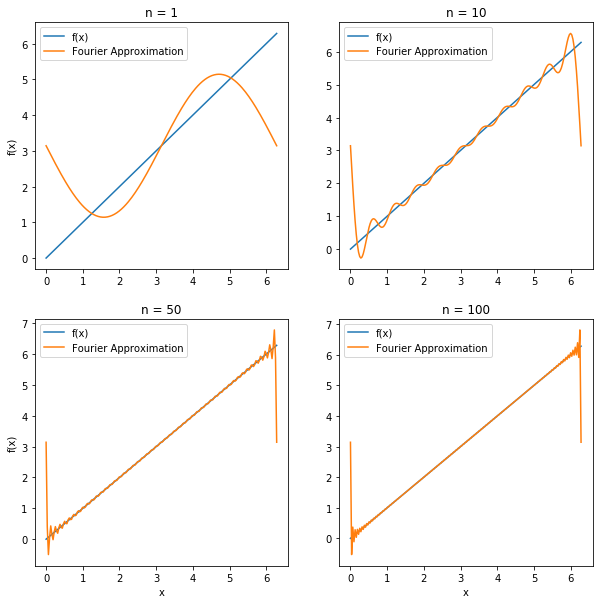
\includegraphics[scale=0.75]{LastOneBOIIISSS.png}

\part Comment on the convergence of the partial Fourier series.
As $n$ goes to $\infty$ the approximation converges to $f(x)$. The approximation becomes acceptable around $n=10$ and is almost equal to $f(x)$ when $n=100$.

\end{parts} 
Note: you should submit only $1$ plot for this problem.

\pagebreak

\question [15] (Denoising a signal) Consider the function $f(x)$ defined as 
\[ f(x) = -\frac15 \left( \frac{x(2\pi-x)}{10}\right)^5 (x + 1.5)(x+2.5)(x-4) + 1.7 \qquad x \in [0,2\pi).\]
\begin{parts}
\part Sample this function at $512$ evenly spaced points to obtain sample values $f_0,\dots,f_{511}$. Add noise to this image as $\tilde{f}_j = f_j + \epsilon r_j$ where $r_j \sim \text{Normal}(0,1)$ and $\epsilon = 10^{-1}$. Plot the sampled function values alongside the noisy function values.
\part Denoise the signal as follows: set all the Fourier coefficients $c_k$ to be zero except for lowest $4$ frequencies. Plot the denoised signal with the original function. 
\part Repeat the previous part, but this time keeping only the lowest $10$ frequencies. 
 \end{parts}
 \begin{lstlisting}[language = Python]
# Function
f = lambda x: (-1/5)*(((x * (2 * math.pi - x))/(10))**5) * (x + 1.5) * (x + 2.5) * (x - 4) + 1.7

# Number of points
n = 512
# Number of coeff
nSmall = 4

# Random noise
noise = np.random.normal(0,1,n)
noise = 0.1 * noise

# Set of evenly spaced points
xs = np.arange(n)*(2*np.pi/n)

# Function values
fs = f(xs) + noise

# Fourier stuff
fk = np.fft.fft(fs)/n
ck = np.fft.fftshift(fk)
k  = np.arange(-n/2,n/2)

# Getting smallest values and update ck
index = heapq.nsmallest(nSmall, enumerate(ck), key=lambda x: x[1])

ckNew = np.zeros(len(ck),dtype=complex)

#ckNew[252] = ck[252]
#ckNew[253] = ck[253]
ckNew[254] = ck[254]
ckNew[255] = ck[255]
ckNew[256] = ck[256]
ckNew[257] = ck[257]
#ckNew[258] = ck[258]
#ckNew[259] = ck[259]
#ckNew[260] = ck[260]
#ckNew[261] = ck[261]


# Fourier stuff
x = np.linspace(0,2*np.pi)
fint = 0*1j*x 
for j in range(n):
  fint += ckNew[j]*np.exp(1j*k[j]*x)

# Plots
fig1, ax1 = plt.subplots()  
  
ax1.plot(xs, f(xs), 'k', linewidth=4)
ax1.plot(xs, f(xs) + noise, 'g-')
ax1.legend({'Original Function', 'Noise'})
ax1.set_xlabel('n')
ax1.set_ylabel('f(x)')
ax1.set_title('Original function and function with noise')

fig2, ax2 = plt.subplots()

ax2.plot(xs, f(xs) + noise, 'k', linewidth = 4)
ax2.plot(x, np.real(fint), 'r', linewidth = 2)
ax2.legend({'True','Interpolated'})
ax2.set_xlabel('n')
ax2.set_ylabel('f(x)')
ax2.set_title('Fourier interpolate and denoised fourier interpolate, %s coeff' % nSmall)
\end{lstlisting}
Note: you should submit $3$ plots for this problem.
\\
\centering
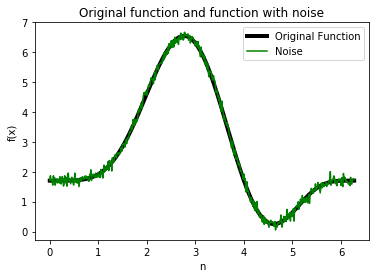
\includegraphics[scale=0.55]{Good_Stuff.png}
\\
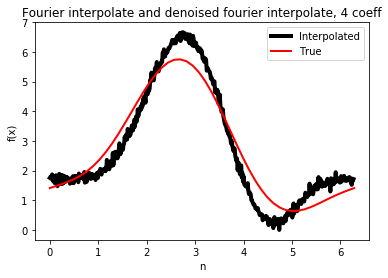
\includegraphics[scale=0.55]{Oh_Baby.png}
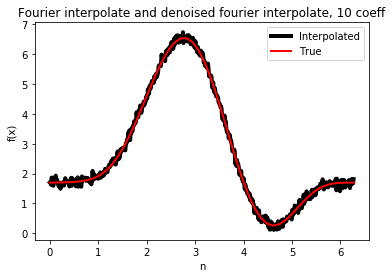
\includegraphics[scale=0.55]{A_Triple_Plot.png}

\pagebreak

\question [15] Consider the function $f(x)$ defined as 
\[ f(x) = 2\pi x -x^2  \qquad x \in [0,2\pi).\]
\begin{parts}
\part Compute the Fourier interpolant $p(x) = \sum_{k=-n/2}^{n/2-1}c_ke^{ikx}$. Plot the interpolant with the original function for $n=8,16,32,64$ points.
\begin{center}
    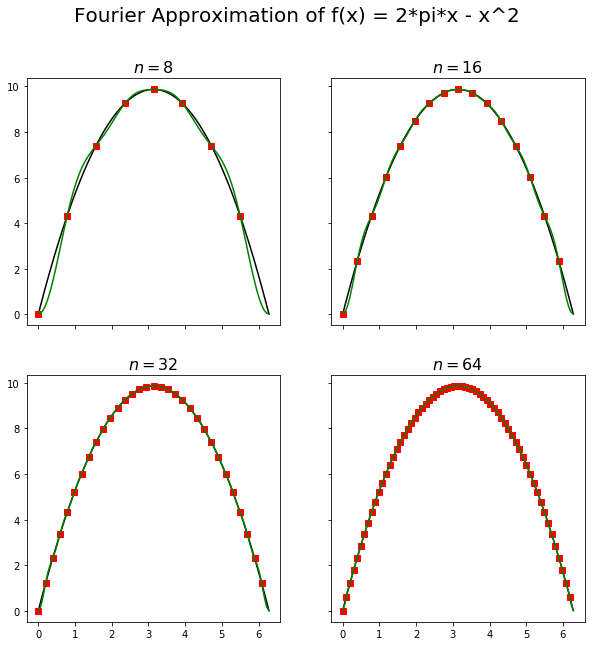
\includegraphics[scale=0.5]{cool1.png}
\end{center}

\begin{lstlisting}[language = Python]
import numpy as np
import pylab as p


x = np.linspace(0, 2*np.pi, 100)

def f(x):
  y = 2*np.pi*x - x**2
  return y

fig, axarray = p.subplots(2,2, sharex = True, sharey = True, figsize = (10,10))
fig.suptitle('Fourier Approximation of f(x) = 2*pi*x - x^2', fontsize = 20)

nlst = [8, 16, 32, 64]
for n, ax in zip(nlst, axarray.flatten()):
  xs = np.arange(n)*(2*np.pi/n)

  fk = np.fft.fft(f(xs))/float(n)
  ck = np.fft.fftshift(fk)
  k  = np.arange(-n/2,n/2)

  fint = 0*1j*x ;
  for i in range(n):
      fint += ck[i]*np.exp(1j*k[i]*x)

  ax.plot(x, f(x), 'k-')
  ax.plot(xs, f(xs), 'rs')
  ax.plot(x, np.real(fint), 'g-')
  ax.set_title('$n = $' + str(n), fontsize = 16)
\end{lstlisting}



\pagebreak

\part Compute the derivative of the interpolant $p'(x)$. Plot this derivative against the true derivative for $n=8,16,32,64$ points.

\begin{center}
    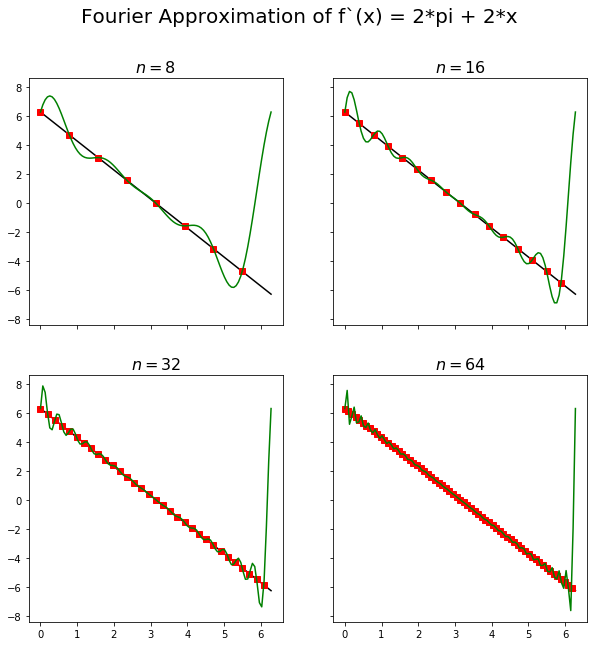
\includegraphics[scale=0.5]{cool2.png}
\end{center}

\begin{lstlisting}[language = Python]
import numpy as np
import pylab as p

x = np.linspace(0, 2*np.pi, 100)

def f(x):
  y = 2*np.pi - 2*x
  return y

fig, axarray = p.subplots(2,2, sharex = True, sharey = True, figsize = (10,10))
fig.suptitle('Fourier Approximation of f`(x) = 2*pi - 2*x', fontsize = 20)

nlst = [8, 16, 32, 64]
for n, ax in zip(nlst, axarray.flatten()):
  xs = np.arange(n)*(2*np.pi/n)

  fk = np.fft.fft(f(xs))/float(n)
  ck = np.fft.fftshift(fk)
  k  = np.arange(-n/2,n/2)

  fint = 0*1j*x ;
  for i in range(n):
      fint += ck[i]*np.exp(1j*k[i]*x)

  ax.plot(x, f(x), 'k-')
  ax.plot(xs, f(xs), 'rs')
  ax.plot(x, np.real(fint), 'g-')
  ax.set_title('$n = $' + str(n), fontsize = 16)
\end{lstlisting}

\part Comment on the accuracy of the Fourier series in parts (a) and (b).

\vspace{5mm}
The approximation for part (a) works pretty well even at small n's due to the nature of the continuity of the f. In part (b) the approximation is a little weird due to the discontinuity of f'. They both have issues at the edges of the functions but that is to be expected.
\vspace{5mm}
 \end{parts}
 
 
Note: you should submit $2$ plots for this problem.

\end{questions}
\end{document}


